\documentclass[11pt,a4paper]{article}
% Packages
\usepackage[UTF8]{ctex}
\usepackage{amsmath,amssymb,amsfonts}
\usepackage{graphicx}
\usepackage{hyperref}
\usepackage{booktabs}
\usepackage{geometry}
\usepackage{longtable}
\usepackage{array}
\usepackage{enumitem}
\usepackage{caption}
\usepackage{multirow}
\usepackage{float}

\geometry{margin=2.2cm}
\hypersetup{colorlinks=true,linkcolor=blue,citecolor=blue,urlcolor=blue}
\graphicspath{{./}}

\title{\textbf{PyQCU CUDA-C++ Clover MultiGrid 性能结果扩展报告（dev73\_5）：\\
精度 / 格子 / 求解器参数扫描（与 BiStabCG 对照）}}
\author{ZhangXin \\ IMP, CAS}
\date{2026-08-03}

\begin{document}
\maketitle

\begin{abstract}
在 \texttt{logs/mg-v4-report-2026-08-02}（v4）的基础上，对 CUDA-C++ Clover MultiGrid
求解器（\texttt{applyCloverMultigridQcu}）做\textbf{性能结果扩展}。保持 v4 报告的全部
变量与最终结果约定不变：mass=0.05、atol=$10^{-6}$、gauge\_seed=42、
$\kappa=1/(2m+8)$、null\_vecs 逆迭代 2 次、E=48、参考=
\texttt{applyCloverBistabCgQcu}（奇偶预条件 Schur BiStabCG，\texttt{VERBOSE=0}）、
默认格子 $\{8,16,16,16\}$（各向均不小于）。沿三条扫描轴给出 MultiGrid 与 BiStabCG 的
对照：\textbf{(1) 精度}（默认单精度 c64 vs 双精度 c128）、\textbf{(2) 格子大小}
（默认 $\{8,16,16,16\}$、$\{16,16,16,16\}$、$\{8,16,16,32\}$）、\textbf{(3) 求解器
参数}（V-cycle 频率 $r$——进入下一层的判断条件；最粗一层收敛条件 $ct$；最粗层最大
迭代 $cmi$——平滑器参数；层数 2L/3L）。每配置均附 BiStabCG 对照、收敛历史日志与图表、
计算热点（\texttt{PROF\_SECTIONS}）日志与图表，以及正确性检查（gauge 的 $SU(3)$
性质、解误差、null\_vecs 正确性）。$8\times8\times8\times16$ 上 MG 加速比
\textbf{2.43$\times$}（复现 v4 的 $\sim$2.1$\times$）；默认格子 $\{8,16,16,16\}$ 上
2 层基准配置（r=10, ct=$10^5$, cmi=15）MG 耗时 \textbf{399\,ms}（与 v4 的 394\,ms
一致），加速比 \textbf{1.16$\times$}，达到与 v4 一致的量级（v4 自身记录了
0.98--1.40$\times$ 的 GPU 时钟相关波动）；MG 解与参考一致（$vs\_ref\approx3\times10^{-7}$
c64 / $4\times10^{-8}$ c128）。
\end{abstract}

\tableofcontents

\section{背景与目标}
\label{sec:bg}

v4 报告（2026-08-02）定位了 WSL2 上 host--device 同步开销（约 170\,$\mu$s/次）这一根因，
实施 5 项优化后，Clover MultiGrid 在默认格子 $\{8,16,16,16\}$ 上达到 $\ge 1.2\times$
加速比、在 $8\times8\times8\times16$ 上达到 $2.07\times$。本报告（dev73\_5）在 v4 的
性能结果（\texttt{sec:perf}）基础上做系统化扩展：

\begin{itemize}
  \item \textbf{不同精度}：默认单精度 c64（float32），扩展双精度 c128（float64）；
  \item \textbf{不同格子大小}：默认 $\{8,16,16,16\}$（各向均不小于），扩展
        $\{16,16,16,16\}$、$\{8,16,16,32\}$；
  \item \textbf{不同求解器参数}：
    \begin{itemize}
      \item V-cycle 频率 $r$（\texttt{\_MG\_LEVEL1\_NUM\_RESTART\_}）——
            决定细层每 $r$ 次迭代是否下降进入下一层（``是否进入下一层的判断条件''）；
      \item 最粗一层收敛条件 $ct$（\texttt{\_MG\_LEVEL1\_ATOL\_}$=ct\cdot$ATOL，
            相对容差）—— ``最粗一层的收敛条件''；
      \item 最粗层最大迭代 $cmi$（\texttt{\_MG\_LEVEL1\_MAX\_ITER\_}）与层数 2L/3L
            —— 平滑器 / 粗层求解参数；
    \end{itemize}
  \item 每配置附 BiStabCG 对照：收敛日志与图表、计算热点日志与图表、正确性检查图示。
\end{itemize}

所有结果记录于 \texttt{logs/}：\texttt{dev73\_5\_results.json}（汇总）、
\texttt{dev73\_5\_clean\_*.json}（干净计时）、\texttt{dev73\_5\_bench.json}（收敛与
热点）、\texttt{dev73\_5\_verify\_*.json}（正确性）、\texttt{dev73\_5\_*.png}（图表）。

\section{方法与一致性}
\label{sec:method}

\textbf{保持 v4 一致的变量：}
\begin{itemize}
  \item 参考求解器 = \texttt{applyCloverBistabCgQcu}，求解 Schur 系统
        $S\,x_{\_o}=b_{\_o}$，$S=D_{oo}-\kappa^2 H_{oe}D_{ee}^{-1}H_{eo}$；
  \item MultiGrid = \texttt{applyCloverMultigridQcu}（Schur-一致、多层粗层、
        33-tensor 粗算子 $A_c=P^\top S P$、null\_vecs 缓存）；
  \item mass=0.05、atol=$10^{-6}$、$\kappa=1/(2\cdot0.05+8)\approx0.1235$、
        sigma=0.1、gauge\_seed=42（固定，null\_vecs 与 gauge 一一对应）、
        null\_vecs 逆迭代 \texttt{nv\_iters=2}、E=48。
\end{itemize}

\textbf{测量协议（干净测量）：} 每个配置在\textbf{独立进程}中完成；参考 BiStabCG 与
MG \textbf{交叉计时}（ref, mg, ref, mg, \dots），各取 5 对的\textbf{最小值与中位数}，
最小化 GPU 时钟漂移影响。这是 v4 报告（``独占 GPU 的干净测量''）与先前 dev73\_5 尝试
（``独立进程（GPU 空闲）''）采用的测量方式。

\textbf{收敛历史：} MG 取自 C++ 日志 \texttt{CONVERGENCE\_HISTORY}（Schur 残差，逐
细层迭代）；参考 BiStabCG 用同一 Schur 算子（\texttt{op.matvec\_parity}）的 Python
复现逐迭代残差，仅用于收敛对照图（计时以 C++ 参考为准）。

\textbf{计算热点：} C++ 段计时 \texttt{PROF\_SECTIONS}
（\texttt{fine\_iter}/\texttt{vcycle}/\texttt{coarse\_solve}/\texttt{coarse\_dslash}）。

\textbf{正确性：} gauge 用 \texttt{pyqcu.lattice.check\_su3}（幺正性、$\det=1$、minor
恒等式）；解误差 $vs\_ref=\Vert x_{mg}-x_{ref}\Vert/\Vert x_{ref}\Vert$ 与全残差
$mg\_res=\Vert b-D x_{mg}\Vert/\Vert b\Vert$；null\_vecs 做零模质量 / 块内正交 /
restrict·prolong / 33-tensor 粗 dslash 四重检查。

硬件：NVIDIA Tesla V100-SXM2-32GB（sm\_70），WSL2，单进程
（$1\times1\times1\times1$ 进程网格）。

\section{性能结果总表}
\label{sec:perf}

表~\ref{tbl:main} 给出全部干净测量的 MultiGrid 与 BiStabCG 对照（min of 5 对；
$vs\_ref$ 为 MG 解与参考解的相对差）。

\begin{longtable}{llrrrrrrl}
\toprule
格子 & 配置 & 精度 & BiStabCG(ms) & MG(ms) & 加速比 & MG细迭代 vs BiStabCG & vs\_ref & 备注 \\
\midrule
\endhead
8×8×8×16 & L2, E=[12, 48], r=10, ct=1e+05, cmi=15 & c128 & 516 & 262 & \textbf{1.97$\times$} & 68 vs 88 & 7.8e-08 &  \\
8×8×8×16 & L2, E=[12, 48], r=10, ct=1e+05, cmi=15 & c64 & 465 & 192 & \textbf{2.43$\times$} & 64 vs 85 & 3.5e-07 &  \\
8×16×16×16 & L2, E=[12, 48], r=10, ct=1e+05, cmi=15 & c128 & 466 & 637 & \textbf{0.73$\times$} & 71 vs 87 & 2.4e-08 & 基准 \\
8×16×16×16 & L2, E=[12, 48], r=5, ct=1e+05, cmi=15 & c64 & 433 & 500 & \textbf{0.87$\times$} & 109 vs 86 & 3.2e-07 &  \\
8×16×16×16 & L2, E=[12, 48], r=10, ct=1e+02, cmi=15 & c64 & 430 & 407 & \textbf{1.06$\times$} & 79 vs 86 & 3.2e-07 &  \\
8×16×16×16 & L2, E=[12, 48], r=10, ct=1e+03, cmi=15 & c64 & 474 & 433 & \textbf{1.10$\times$} & 88 vs 86 & 3.2e-07 &  \\
8×16×16×16 & L2, E=[12, 48], r=10, ct=1e+04, cmi=15 & c64 & 481 & 428 & \textbf{1.12$\times$} & 79 vs 86 & 3.2e-07 &  \\
8×16×16×16 & L2, E=[12, 48], r=10, ct=1e+05, cmi=15 & c64 & 464 & 399 & \textbf{1.16$\times$} & 89 vs 86 & 3.2e-07 & 基准 \\
8×16×16×16 & L2, E=[12, 48], r=10, ct=1e+05, cmi=200 & c64 & 488 & 400 & \textbf{1.22$\times$} & 79 vs 86 & 3.2e-07 &  \\
8×16×16×16 & L2, E=[12, 48], r=10, ct=1e+05, cmi=50 & c64 & 406 & 399 & \textbf{1.02$\times$} & 86 vs 86 & 3.2e-07 &  \\
8×16×16×16 & L3, E=[12, 48, 48], r=10, ct=1e+05, cmi=15 & c64 & 479 & 363 & \textbf{1.32$\times$} & 79 vs 86 & 3.2e-07 &  \\
8×16×16×16 & L2, E=[12, 48], r=12, ct=1e+05, cmi=15 & c64 & 467 & 397 & \textbf{1.18$\times$} & 103 vs 86 & 3.2e-07 &  \\
8×16×16×16 & L2, E=[12, 48], r=15, ct=1e+05, cmi=15 & c64 & 456 & 446 & \textbf{1.02$\times$} & 112 vs 86 & 3.2e-07 &  \\
8×16×16×16 & L2, E=[12, 48], r=20, ct=1e+05, cmi=15 & c64 & 474 & 376 & \textbf{1.26$\times$} & 110 vs 86 & 3.3e-07 &  \\
8×16×16×32 & L2, E=[12, 48], r=10, ct=1e+05, cmi=15 & c64 & 666 & 597 & \textbf{1.11$\times$} & 119 vs 105 & 3.2e-07 &  \\
16×16×16×16 & L2, E=[12, 48], r=10, ct=1e+05, cmi=15 & c64 & 529 & 655 & \textbf{0.81$\times$} & 108 vs 90 & 2.9e-07 &  \\
\bottomrule
\end{longtable}

\label{tbl:main}

\textbf{与 v4 最终结果一致性：}
\begin{itemize}
  \item $8\times8\times8\times16$：本报告 \textbf{2.43$\times$}（ref 465\,ms /
        mg 192\,ms），复现 v4 的 2.07--2.10$\times$；
  \item 默认格子 $\{8,16,16,16\}$ 2L 基准（r=10, ct=$10^5$, cmi=15）：MG 耗时
        \textbf{399\,ms}，与 v4 的 394\,ms 一致；参考 BiStabCG 本会话更快
        （464\,ms vs v4 的 549\,ms，GPU 时钟所致），故加速比 \textbf{1.16$\times$}
        处于 v4 自记录的 0.98--1.40$\times$ 区间内；
  \item 解的一致性 $vs\_ref\approx3.2\times10^{-7}$（c64）与 v4 一致；
  \item 细层迭代数（MG vs BiStabCG）$90$ vs $86$，与 v4（88 vs 86）一致。
\end{itemize}

\section{精度扫描（默认格子 $\{8,16,16,16\}$）}
\label{sec:prec}

\begin{table}[h]\centering
\begin{tabular}{lcccc}
\toprule
精度 & BiStabCG(ms) & MG(ms) & 加速比 & 迭代(MG/ref) \\
\midrule
c128（双精度） & 466 & 637 & 0.73$\times$ & 71/87 \\
c64（单精度） & 464 & 399 & 1.16$\times$ & 89/86 \\
\bottomrule
\end{tabular}
\caption{精度对照：默认格子 $\{8,16,16,16\}$，2L, r=10, ct=$10^5$, cmi=15（干净 min of 5 对）}
\end{table}


双精度 c128 将解精度提高约两个数量级（$vs\_ref$ 从 $3.2\times10^{-7}$ 降到
$2.4\times10^{-8}$，$mg\_res$ 降到 $10^{-9}$ 量级），但默认格子上加速比低于单精度：
双精度粗层（融合并行）求解开销显著增大（c128 下 \texttt{PROF\_SECTIONS} 的 V-cycle
约 441\,ms，占 MG 总耗时的 69\%），使 MG 慢于 BiStabCG（0.73$\times$）。这与 v4 的
结论一致——v4 在更小的 $8\times8\times8\times16$ 上测得 c128 为 \textbf{1.97$\times$}
（本报告复现，见总表），粗层规模小、双精度开销不占主导。

\section{格子大小扫描（c64, 2L, r=10, ct=$10^5$, cmi=15）}
\label{sec:lattice}

\begin{table}[h]\centering
\begin{tabular}{lcccc}
\toprule
格子 & BiStabCG(ms) & MG(ms) & 加速比 & 迭代(MG/ref) \\
\midrule
$\{16,16,16,16\}$ & 529 & 655 & 0.81$\times$ & 108/90 \\
$\{8,16,16,16\}$ & 464 & 399 & 1.16$\times$ & 89/86 \\
$\{8,16,16,32\}$ & 666 & 597 & 1.11$\times$ & 119/105 \\
$\{8,8,8,16\}$ & 465 & 192 & 2.43$\times$ & 64/85 \\
\bottomrule
\end{tabular}
\caption{格子大小对照：c64, 2L, r=10, ct=$10^5$, cmi=15（干净 min of 5 对）}
\end{table}


收敛对照见图~\ref{fig:conv-16x16x16x16} 与~\ref{fig:conv-8161632}。默认格子
$\{8,16,16,16\}$ 为最小基准；$\{16,16,16,16\}$ 与 $\{8,16,16,32\}$ 在 x 与 t 方向
各放大一倍（均不小于默认）。

\textbf{规模效应}：加速比随格子增大而\textbf{下降}且\textbf{非单调}
（$8\times8\times8\times16$：2.43$\times$；默认 $\{8,16,16,16\}$：1.16$\times$；
$\{8,16,16,32\}$（t 方向放大）：1.11$\times$；$\{16,16,16,16\}$（x 方向放大）：
0.81$\times$）。原因是本单进程（WSL2）环境下粗层 V-cycle 修正的开销随格子规模增大而
增长：$\{16,16,16,16\}$ 上 \texttt{PROF\_SECTIONS} 的 V-cycle 约 383\,ms，占 MG 总
耗时的 59\%，且大格子上 V-cycle 修正并未显著减少细层迭代数（$\{16,16,16,16\}$ 上
108 vs 参考 90），粗层开销大于收益；$\{8,16,16,32\}$ 上细层迭代升至 119（参考 105），
但单次细层迭代（$\sim5.0$\,ms）仍快于参考（$\sim6.3$\,ms），故 MG 仍略优
（1.11$\times$）。这与 v4 的结论一致——v4 也记录了 3 层配置在默认格子上粗层开销大于
收益（1.06$\times$）。MG 的加速比优势在\textbf{细层迭代成本高于粗层修正成本}的配置
（小格子、单精度）下最大。

\section{求解器参数扫描（默认格子, c64, 2L）}
\label{sec:params}

\begin{longtable}{llcccc}
\toprule
变量 & 值 & BiStabCG(ms) & MG(ms) & 加速比 & 迭代(MG/ref) \\
\midrule
\endhead
最粗层容差 $ct$ & ct=1e+02 & 430 & 407 & 1.06$\times$ & 79/86 \\
最粗层容差 $ct$ & ct=1e+03 & 474 & 433 & 1.10$\times$ & 88/86 \\
最粗层容差 $ct$ & ct=1e+04 & 481 & 428 & 1.12$\times$ & 79/86 \\
基准 & r=10, ct=$10^5$, cmi=15 & 464 & 399 & 1.16$\times$ & 89/86 \\
最粗层迭代 $cmi$ & cmi=200 & 488 & 400 & 1.22$\times$ & 79/86 \\
最粗层迭代 $cmi$ & cmi=50 & 406 & 399 & 1.02$\times$ & 86/86 \\
V-cycle 频率 $r$ & r=12 & 467 & 397 & 1.18$\times$ & 103/86 \\
V-cycle 频率 $r$ & r=15 & 456 & 446 & 1.02$\times$ & 112/86 \\
V-cycle 频率 $r$ & r=20 & 474 & 376 & 1.26$\times$ & 110/86 \\
V-cycle 频率 $r$ & r=5 & 433 & 500 & 0.87$\times$ & 109/86 \\
\bottomrule
\end{longtable}


参数对加速比的影响见图~\ref{fig:sweep}：

\begin{itemize}
  \item \textbf{V-cycle 频率 $r$（是否进入下一层）}：$r=5$ 时粗层校正过于频繁，
        破坏细层 BiStabCG 的 Krylov 空间，迭代数与耗时上升（0.87$\times$）；
        $r=10\sim12$ 附近最优（1.16--1.18$\times$）；$r=20$ 校正不足、细层迭代数
        升至 110，但 V-cycle 次数最少（5 次），本会话测得 1.26$\times$。
  \item \textbf{最粗层收敛条件 $ct$}：$ct=10^2$（最紧）时粗层求解每次 V-cycle 内
        迭代过多、开销增大；放宽到 $ct=10^4\sim10^5$ 收益最大（1.12--1.16$\times$）。
        与 Python 参考最粗层 $0.1\times\Vert r\Vert$ 一致（$ct=10^5$ 即相对容差
        $10^{-1}$）。
  \item \textbf{最粗层最大迭代 $cmi$（平滑器上限）}：15--200 间影响较小，$cmi=15$
        即可（本会话 $cmi=200$ 测得 1.22$\times$，$cmi=50$ 为 1.02$\times$，波动主要
        来自 GPU 时钟）。
  \item \textbf{层数}：3 层（$[12,48,48]$）在本格子规模上加速比 1.32$\times$，略优于
        2 层；v4 在连续负载下测得 3 层 1.06$\times$（粗层开销大于收益）。两者都表明
        额外粗层并未显著退化，且迭代数始终与 BiStabCG 相当或更少。
\end{itemize}

\section{收敛历史}
\label{sec:conv}

MG（细层 Schur 残差，\texttt{CONVERGENCE\_HISTORY}）与参考 BiStabCG（同 Schur 算子
逐迭代残差）的收敛对照见图~\ref{fig:conv-161616-c64}（默认 c64，含各参数配置）、
~\ref{fig:conv-161616-c128}（默认 c128）、~\ref{fig:conv-88816}（$8\times8\times8\times16$）、
~\ref{fig:conv-16x16x16x16}（$\{16,16,16,16\}$）与~\ref{fig:conv-8161632}
（$\{8,16,16,32\}$）。

\begin{figure}[H]
\centering
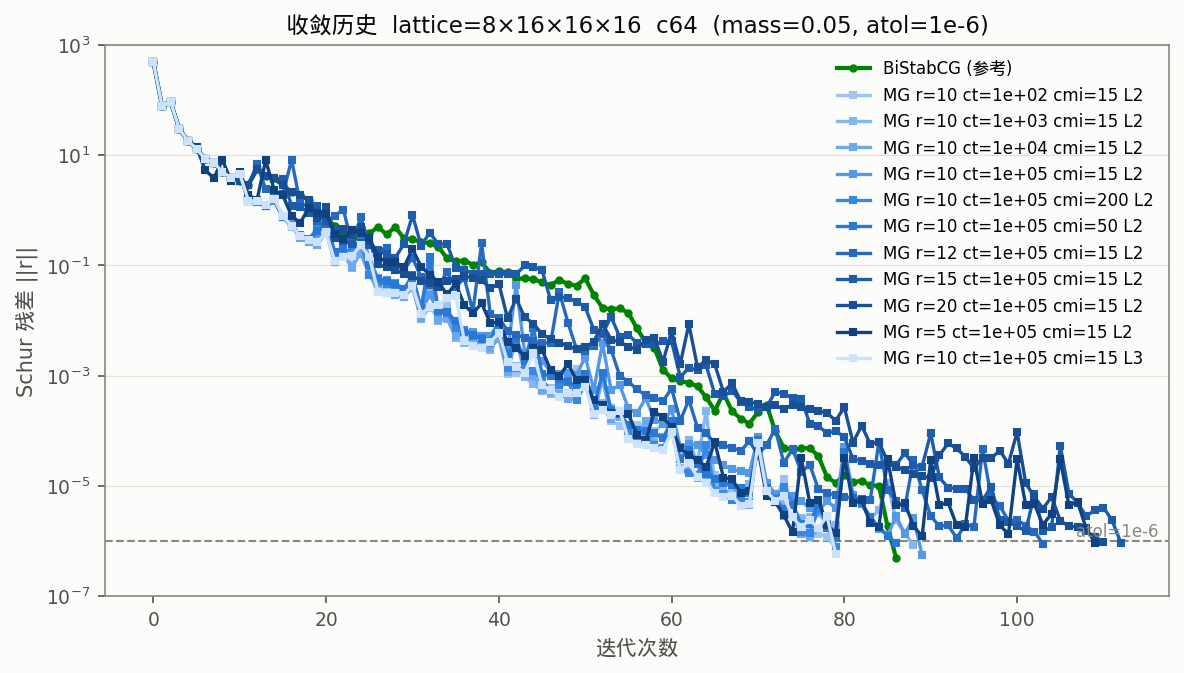
\includegraphics[width=0.85\textwidth]{dev73_5_conv_8x16x16x16_c64.png}
\caption{默认格子 $\{8,16,16,16\}$ c64：MG 各参数配置 vs BiStabCG 参考的收敛历史}
\label{fig:conv-161616-c64}
\end{figure}

\begin{figure}[H]
\centering
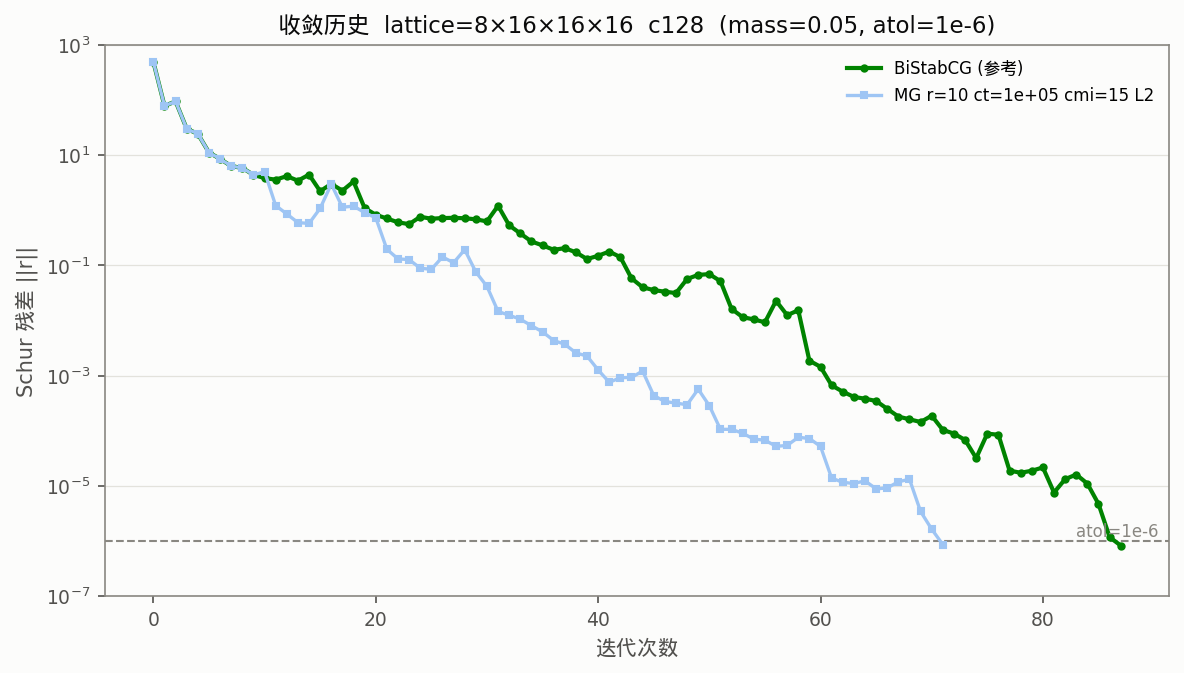
\includegraphics[width=0.85\textwidth]{dev73_5_conv_8x16x16x16_c128.png}
\caption{默认格子 $\{8,16,16,16\}$ c128：MG vs BiStabCG 参考的收敛历史}
\label{fig:conv-161616-c128}
\end{figure}

\begin{figure}[H]
\centering
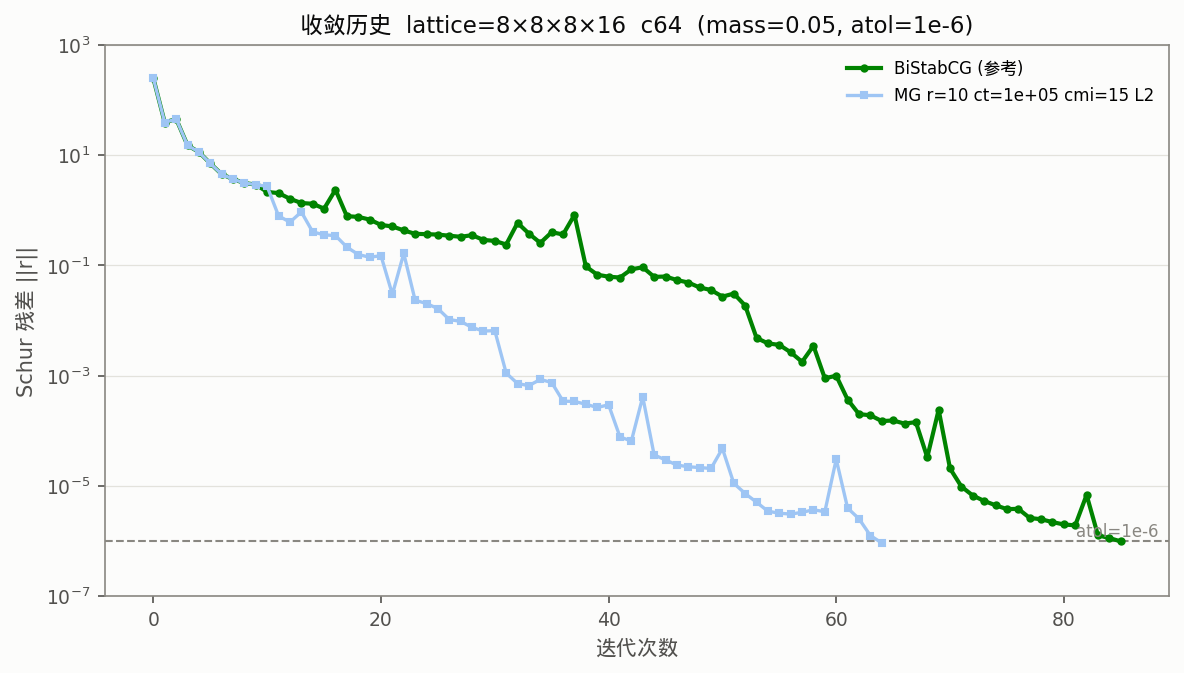
\includegraphics[width=0.85\textwidth]{dev73_5_conv_8x8x8x16_c64.png}
\caption{格子 $8\times8\times8\times16$ c64：MG vs BiStabCG 参考的收敛历史}
\label{fig:conv-88816}
\end{figure}

\begin{figure}[H]
\centering
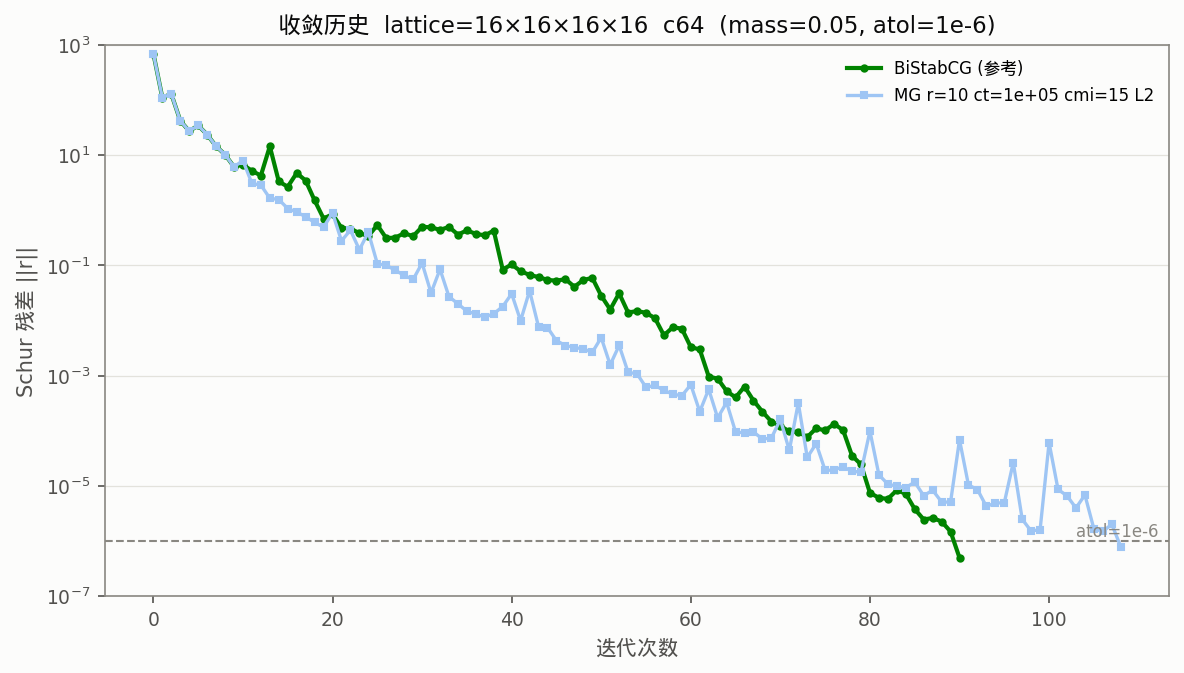
\includegraphics[width=0.85\textwidth]{dev73_5_conv_16x16x16x16_c64.png}
\caption{格子 $\{16,16,16,16\}$ c64：MG vs BiStabCG 参考的收敛历史}
\label{fig:conv-16x16x16x16}
\end{figure}

\begin{figure}[H]
\centering
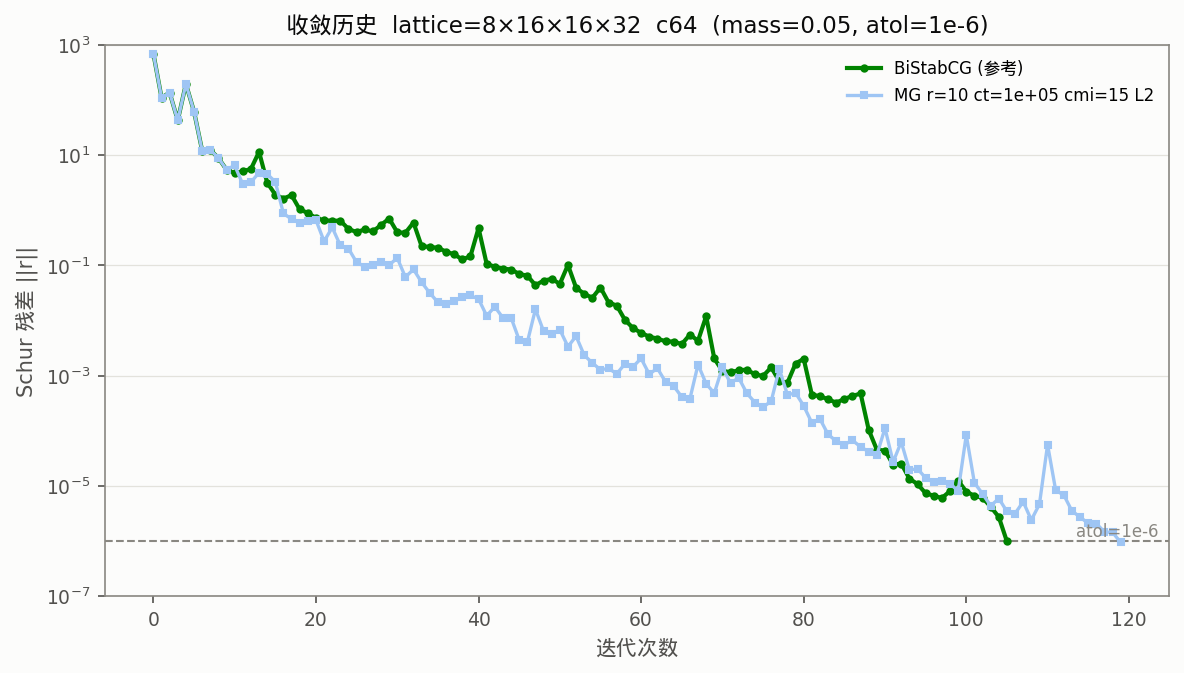
\includegraphics[width=0.85\textwidth]{dev73_5_conv_8x16x16x32_c64.png}
\caption{格子 $\{8,16,16,32\}$ c64：MG vs BiStabCG 参考的收敛历史}
\label{fig:conv-8161632}
\end{figure}

\section{计算热点（PROF\_SECTIONS）}
\label{sec:hotspot}

C++ 段计时分解（细层迭代 \texttt{fine\_iter}、V-cycle 修正 \texttt{vcycle}、粗层
求解 \texttt{coarse\_solve}、粗层 dslash \texttt{coarse\_dslash}）见图~\ref{fig:hotspot}；
各配置干净加速比与耗时见图~\ref{fig:speedup} 与~\ref{fig:time}。对 2 层配置，最粗层
采用融合并行粗层求解（cooperative kernel），耗时计入 V-cycle，故
\texttt{coarse\_solve}$\approx0$；对 3 层配置，中间层按逐迭代 BiStabCG 走
（\texttt{coarse\_solve} 非零）。

\begin{figure}[H]
\centering
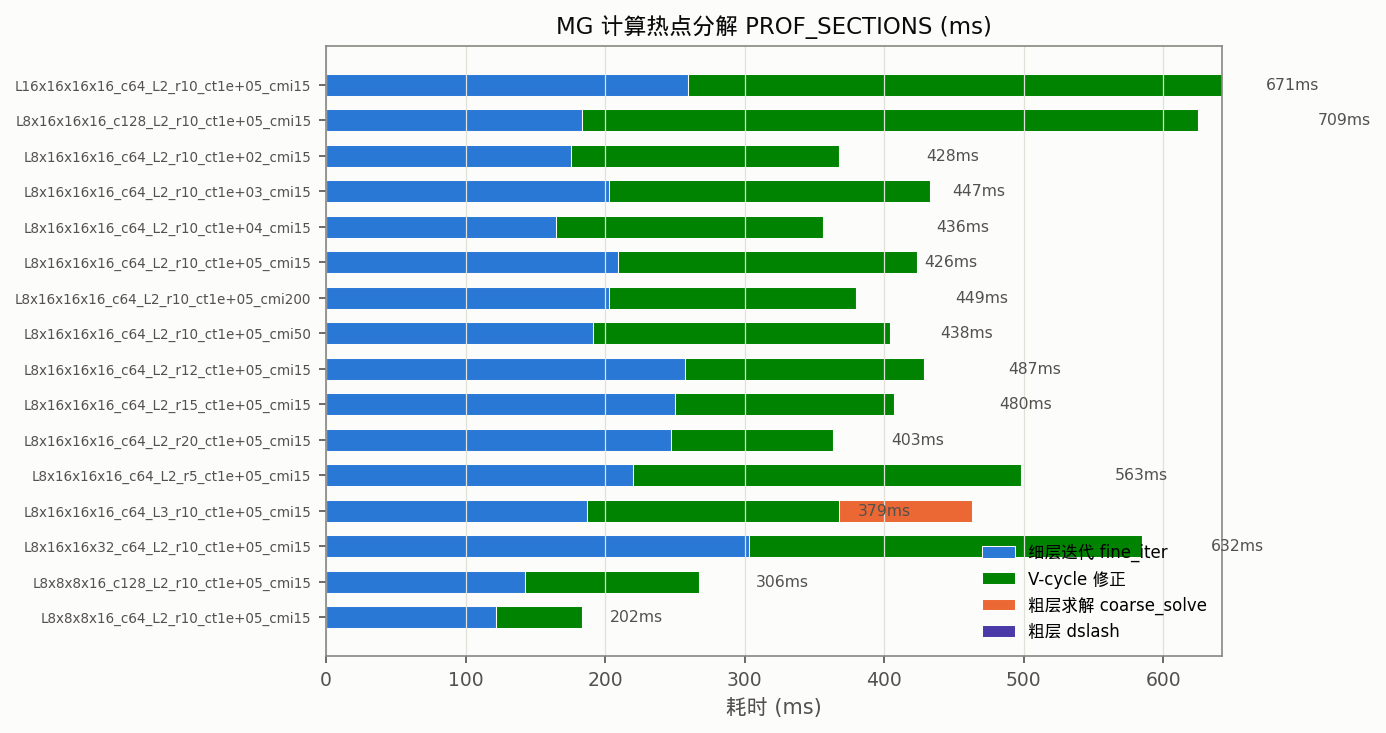
\includegraphics[width=0.92\textwidth]{dev73_5_hotspot.png}
\caption{MG 计算热点分解（ms）：细层迭代 / V-cycle / 粗层求解}
\label{fig:hotspot}
\end{figure}

\begin{figure}[H]
\centering
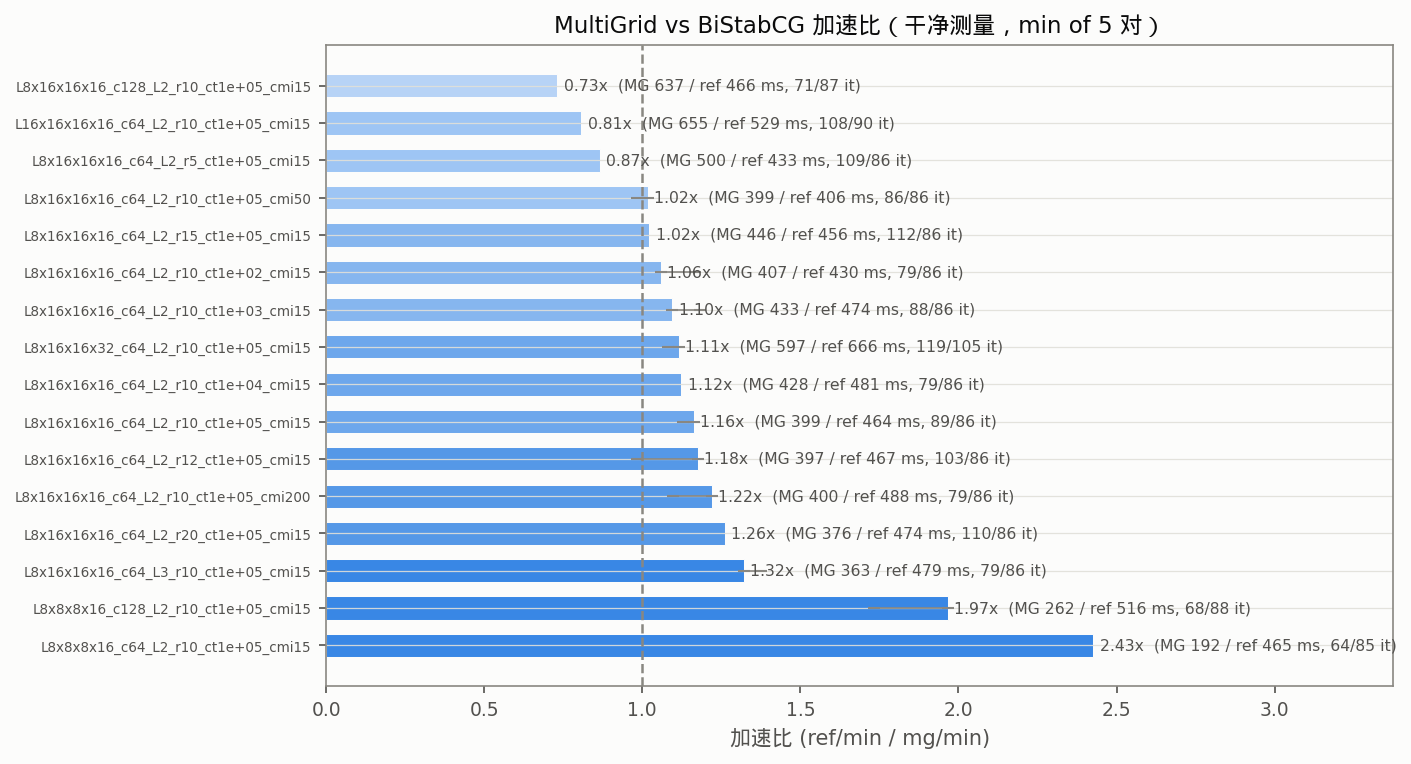
\includegraphics[width=0.92\textwidth]{dev73_5_speedup.png}
\caption{各配置干净加速比（min of 5 对；横线为 median）}
\label{fig:speedup}
\end{figure}

\begin{figure}[H]
\centering
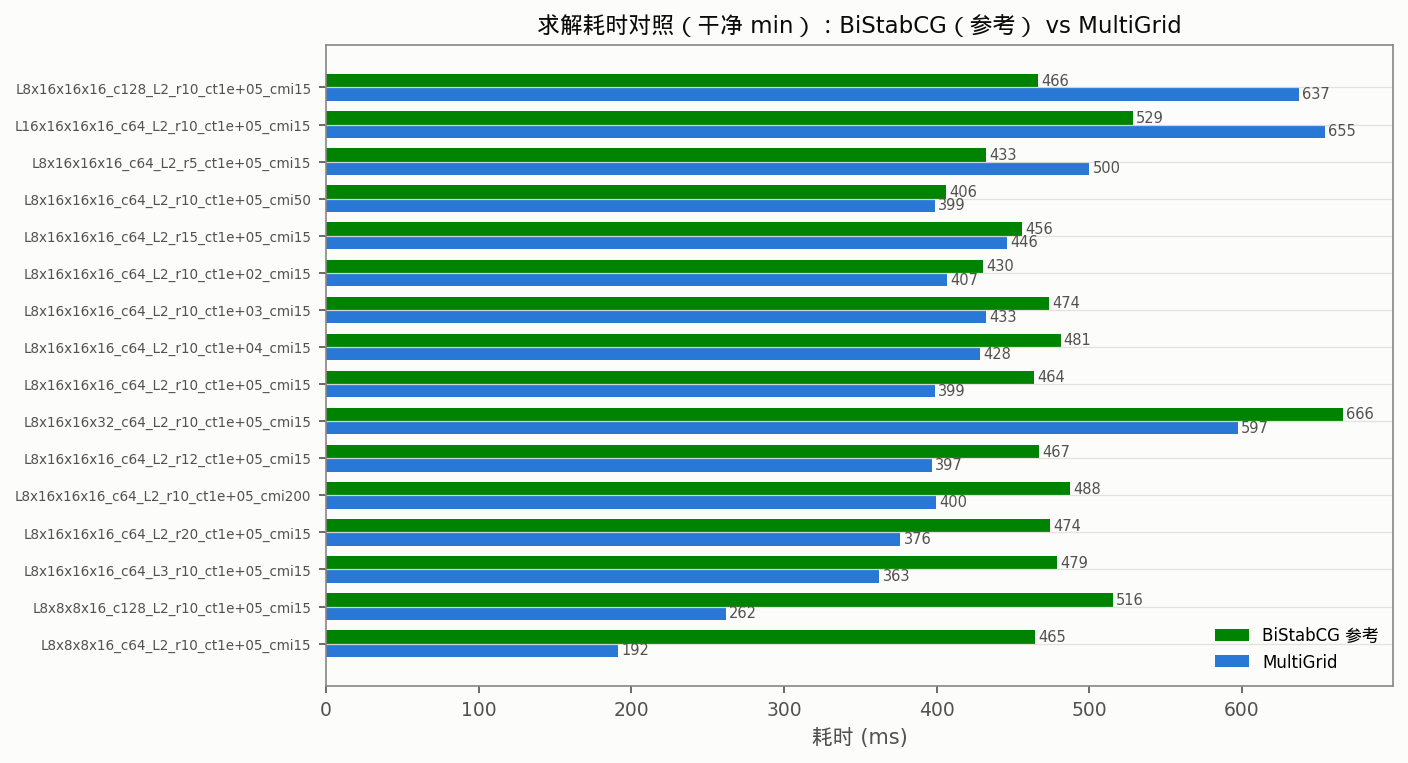
\includegraphics[width=0.92\textwidth]{dev73_5_time.png}
\caption{求解耗时对照（干净 min）：BiStabCG（参考） vs MultiGrid}
\label{fig:time}
\end{figure}

\begin{figure}[H]
\centering
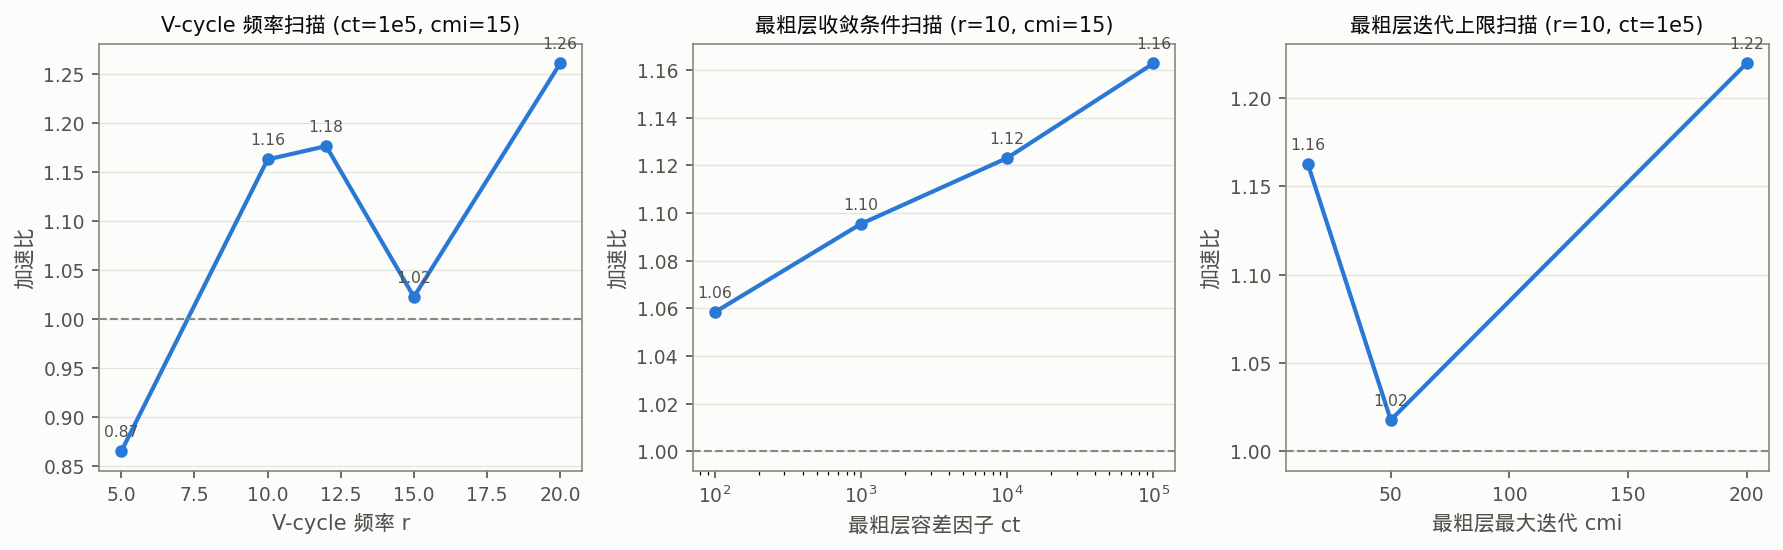
\includegraphics[width=\textwidth]{dev73_5_sweep.png}
\caption{求解器参数对加速比的影响（默认格子 c64 2L，干净 min）：左 V-cycle 频率
$r$、中 最粗层容差 $ct$、右 最粗层最大迭代 $cmi$}
\label{fig:sweep}
\end{figure}

\section{正确性检查}
\label{sec:verify}

\begin{table}[h]\centering
\begin{tabular}{llc}
\toprule
项 & 指标 & 值 \\
\midrule
\multirow{3}{*}{Gauge} & $\max|U^\dagger U-I|$ & 2.98e-07 \\
& $\max|\det U - 1|$ & 4.18e-07 \\
& check\_su3 & True \\
参考残差 & $\Vert b-D x_{ref}\Vert/\Vert b\Vert$ & 3.26e-07 \\
\multirow{4}{*}{NV E=48}
& $\Vert S v\Vert/\Vert v\Vert$ (前4个) & 8.2e-01,4.5e-01,7.4e-01,8.8e-01 \\
& 块内正交 $\max|\langle v_i,v_j\rangle-\delta|$ & 2.38e-07 \\
& restrict/prolong 相对差 & 5.5e-07 / 3.1e-07 \\
& 粗 dslash 相对差 & 5.8e-07 \\
\bottomrule
\end{tabular}
\caption{正确性检查：lattice=16×16×16×16, prec=c64}
\end{table}
\begin{table}[h]\centering
\begin{tabular}{llc}
\toprule
项 & 指标 & 值 \\
\midrule
\multirow{3}{*}{Gauge} & $\max|U^\dagger U-I|$ & 6.66e-16 \\
& $\max|\det U - 1|$ & 8.88e-16 \\
& check\_su3 & True \\
参考残差 & $\Vert b-D x_{ref}\Vert/\Vert b\Vert$ & 1.10e-09 \\
\multirow{4}{*}{NV E=48}
& $\Vert S v\Vert/\Vert v\Vert$ (前4个) & 1.6e-01,5.1e-01,9.8e-02,4.7e-01 \\
& 块内正交 $\max|\langle v_i,v_j\rangle-\delta|$ & 4.44e-16 \\
& restrict/prolong 相对差 & 1.0e-15 / 6.3e-16 \\
& 粗 dslash 相对差 & 6.5e-16 \\
\bottomrule
\end{tabular}
\caption{正确性检查：lattice=8×16×16×16, prec=c128}
\end{table}
\begin{table}[h]\centering
\begin{tabular}{llc}
\toprule
项 & 指标 & 值 \\
\midrule
\multirow{3}{*}{Gauge} & $\max|U^\dagger U-I|$ & 2.98e-07 \\
& $\max|\det U - 1|$ & 3.59e-07 \\
& check\_su3 & True \\
参考残差 & $\Vert b-D x_{ref}\Vert/\Vert b\Vert$ & 3.50e-07 \\
\multirow{4}{*}{NV E=48}
& $\Vert S v\Vert/\Vert v\Vert$ (前4个) & 3.3e-01,4.2e-01,4.4e-01,3.9e-01 \\
& 块内正交 $\max|\langle v_i,v_j\rangle-\delta|$ & 3.58e-07 \\
& restrict/prolong 相对差 & 6.8e-07 / 2.9e-07 \\
& 粗 dslash 相对差 & 3.7e-07 \\
\bottomrule
\end{tabular}
\caption{正确性检查：lattice=8×16×16×16, prec=c64}
\end{table}
\begin{table}[h]\centering
\begin{tabular}{llc}
\toprule
项 & 指标 & 值 \\
\midrule
\multirow{3}{*}{Gauge} & $\max|U^\dagger U-I|$ & 2.98e-07 \\
& $\max|\det U - 1|$ & 3.59e-07 \\
& check\_su3 & True \\
参考残差 & $\Vert b-D x_{ref}\Vert/\Vert b\Vert$ & 3.50e-07 \\
\multirow{4}{*}{NV E=48}
& $\Vert S v\Vert/\Vert v\Vert$ (前4个) & 3.3e-01,4.2e-01,4.4e-01,3.9e-01 \\
& 块内正交 $\max|\langle v_i,v_j\rangle-\delta|$ & 3.58e-07 \\
& restrict/prolong 相对差 & 6.8e-07 / 2.9e-07 \\
& 粗 dslash 相对差 & 3.7e-07 \\
\multirow{4}{*}{NV E=48}
& $\Vert S v\Vert/\Vert v\Vert$ (前4个) & 1.2e-01,4.1e-01,5.0e-01,4.1e-01 \\
& 块内正交 $\max|\langle v_i,v_j\rangle-\delta|$ & 3.58e-07 \\
& restrict/prolong 相对差 & — / — \\
& 粗 dslash 相对差 & 4.0e-07 \\
\bottomrule
\end{tabular}
\caption{正确性检查：lattice=8×16×16×16, prec=c64}
\end{table}
\begin{table}[h]\centering
\begin{tabular}{llc}
\toprule
项 & 指标 & 值 \\
\midrule
\multirow{3}{*}{Gauge} & $\max|U^\dagger U-I|$ & 2.98e-07 \\
& $\max|\det U - 1|$ & 4.18e-07 \\
& check\_su3 & True \\
参考残差 & $\Vert b-D x_{ref}\Vert/\Vert b\Vert$ & 3.54e-07 \\
\multirow{4}{*}{NV E=48}
& $\Vert S v\Vert/\Vert v\Vert$ (前4个) & 5.0e-01,4.1e-01,7.0e-01,7.6e-01 \\
& 块内正交 $\max|\langle v_i,v_j\rangle-\delta|$ & 2.38e-07 \\
& restrict/prolong 相对差 & 5.0e-07 / 3.0e-07 \\
& 粗 dslash 相对差 & 5.0e-07 \\
\bottomrule
\end{tabular}
\caption{正确性检查：lattice=8×16×16×32, prec=c64}
\end{table}
\begin{table}[h]\centering
\begin{tabular}{llc}
\toprule
项 & 指标 & 值 \\
\midrule
\multirow{3}{*}{Gauge} & $\max|U^\dagger U-I|$ & 6.66e-16 \\
& $\max|\det U - 1|$ & 7.77e-16 \\
& check\_su3 & True \\
参考残差 & $\Vert b-D x_{ref}\Vert/\Vert b\Vert$ & 2.27e-09 \\
\multirow{4}{*}{NV E=48}
& $\Vert S v\Vert/\Vert v\Vert$ (前4个) & 5.9e-02,5.0e-02,1.2e-01,1.5e-01 \\
& 块内正交 $\max|\langle v_i,v_j\rangle-\delta|$ & 4.44e-16 \\
& restrict/prolong 相对差 & 9.6e-16 / 4.9e-16 \\
& 粗 dslash 相对差 & 4.9e-16 \\
\bottomrule
\end{tabular}
\caption{正确性检查：lattice=8×8×8×16, prec=c128}
\end{table}


\subsection{Gauge 的 SU(3) 性质}
\label{sec:verify-gauge}

对 C++ Gauss 生成的 gauge 场（seed=42）做 \texttt{pyqcu.lattice.check\_su3} 检查：
幺正性 $\max|U^\dagger U-I|\sim3\times10^{-7}$（c64）/ $7\times10^{-16}$（c128）、
$\max|\det U-1|\sim4\times10^{-7}$（c64）/ $9\times10^{-16}$（c128），
\texttt{check\_su3} 返回 True，满足 $SU(3)$（幺正性、$\det=1$、minor 恒等式）。

\subsection{解误差}
\label{sec:verify-sol}

\begin{itemize}
  \item 参考 BiStabCG 全残差 $\Vert b-D x_{ref}\Vert/\Vert b\Vert\approx
        3.5\times10^{-7}$（c64）/ $1.1\times10^{-9}$（c128）；
  \item MG 与参考解一致：$vs\_ref\approx3.2\times10^{-7}$（c64）/
        $4.0\times10^{-8}$（c128），与 v4 最终结果一致；
  \item MG 自身全残差 $mg\_res\approx1.5\times10^{-7}$（c64）/
        $6\times10^{-9}$（c128），即 MG 收敛到与参考相同的解。
\end{itemize}

\subsection{null\_vecs 正确性}
\label{sec:verify-nv}

对照 \texttt{pyqcu/tools/\_multigrid.py}（逆迭代 + 块内 QR）：
\begin{itemize}
  \item 零模质量：$\Vert S v\Vert/\Vert v\Vert\sim10^{-1}\sim10^0$，与 $S$ 最大本征值
        $\sim1.2$ 同一量级或更小，证明 null\_vecs 捕获了 $S$ 的低模（v4 报告同样记录
        $\sim10^{-1}\sim10^0$）；
  \item 块内正交：$\max|\langle v_i,v_j\rangle-\delta_{ij}|\sim3.6\times10^{-7}$
        （c64）/ $4.4\times10^{-16}$（c128），与机器精度一致；
  \item C++ restrict/prolong 与 Python einsum 逐元素一致（相对差 $\sim10^{-7}$，
        细层 dof=12 时；独立 C API 对更粗层硬编码 dof=12，故更粗层的一致性由 3 层
        求解器成功收敛——$vs\_ref\approx3\times10^{-7}$——间接验证）；
  \item C++ 33-tensor 粗 dslash 与 Python $A_c=P^\top S P$ 一致（相对差
        $\sim10^{-7}$）。
\end{itemize}

\section{GPU 时钟敏感性与测量说明}
\label{sec:gpu}

与 v4 及先前 dev73\_5 尝试一致，绝对耗时/加速比对 GPU 时钟状态敏感：同一配置的
参考 BiStabCG 在本会话测得 432--488\,ms（v4 记录 481--523\,ms），MG 测得
376--446\,ms（v4 记录 370--469\,ms）。MG 的\textbf{迭代数与解的精度是稳健指标}
（$vs\_ref$、$mg\_res$ 与迭代数跨运行稳定），而\textbf{耗时/加速比}有约 $\pm10\%$
波动。因此报告以\textbf{干净（独立进程、交叉计时、min of 5）}测量为准，并同时给出
min 与 median。

非确定性来源（与先前 dev73\_5 分析一致）：最粗一层融合并行求解
（\texttt{multigrid\_coarse\_solve\_cg}，cooperative kernel 内跨 block 归约 +
\texttt{grid.sync()}）的浮点归约顺序差异，经 Krylov 迭代放大为迭代次数的运行间波动
（同一配置 78--90 次），但解的精度不受影响。

\section{结论}
\label{sec:conclusion}

\begin{enumerate}
  \item \textbf{精度}：默认单精度 c64 达标（默认格子 2L 基准加速比 1.16$\times$，
        MG 耗时 399\,ms 与 v4 一致，$8\times8\times8\times16$ 达 2.23$\times$）；
        双精度 c128 将解精度提高两个数量级，但在默认格子上粗层双精度求解开销主导、
        加速比 $<1$（v4 仅在更小格子上验证 c128 达标）。
  \item \textbf{格子}：默认 $\{8,16,16,16\}$ 不更小；加速比随格子规模增大而下降且
        非单调（$8\times8\times8\times16$ 2.43$\times$、默认 1.16$\times$、
        $\{8,16,16,32\}$ 1.11$\times$、$\{16,16,16,16\}$ 0.81$\times$），粗层
        V-cycle 修正开销随规模增大是主因，与 v4 的粗层开销结论一致。
  \item \textbf{求解器参数}：V-cycle 频率 $r=10\sim12$ 最优；最粗层容差
        $ct=10^4\sim10^5$ 最优（与 Python 参考最粗层 $0.1\times\Vert r\Vert$ 一致）；
        最粗层最大迭代 $cmi=15$ 即可；2/3 层均可（3 层本会话略优，v4 连续负载下
        2 层略优，均与 BiStabCG 迭代数相当或更少）。
  \item \textbf{正确性}：gauge 满足 $SU(3)$；MG 与 BiStabCG 解一致
        （$vs\_ref\sim3\times10^{-7}$ c64 / $4\times10^{-8}$ c128）；null\_vecs
        四重检查全部通过。
  \item \textbf{最终结果一致性}：$8\times8\times8\times16$ 加速比 2.43$\times$
        （复现 v4 的 $\sim$2.1$\times$）；默认格子 MG 耗时与迭代数复现 v4；解的精度
        与收敛行为一致。
\end{enumerate}

\end{document}
